%%%%%%%%%%%%%%%%%%%%%%%%%%%%%%%%%%%%%%%%%%%%%%%%%%%%%%%%%%%%%%%%%%%%
%% I, the copyright holder of this work, release this work into the
%% public domain. This applies worldwide. In some countries this may
%% not be legally possible; if so: I grant anyone the right to use
%% this work for any purpose, without any conditions, unless such
%% conditions are required by law.
%%%%%%%%%%%%%%%%%%%%%%%%%%%%%%%%%%%%%%%%%%%%%%%%%%%%%%%%%%%%%%%%%%%%

% This theme was based on fibeamer theme 
% If you found any bugs please contact @karlosos
% This repository is hosted on github https://github.com/karlosos/zut-fibeamer/

\documentclass{beamer}
\usetheme[faculty=wi]{fibeamer}
\usepackage[utf8]{inputenc}
\usepackage[
  main=polish,
  polish
]{babel}

\title{Aula 2  - Projetos NodeJs}
\subtitle{Tópicos especiais em Sistemas}
\author{Prof. Juliana Costa Silva - juliana.silva@up.edu.br}

\usepackage{ragged2e}  % `\justifying` text
\usepackage{booktabs}  % Tables
\usepackage{tabularx}
\usepackage{tikz}      % Diagrams
\usetikzlibrary{calc, shapes, backgrounds}
\usepackage{amsmath, amssymb}
\usepackage{url}       % `\url`s
\usepackage{listings}  % Code listings
\frenchspacing
\begin{document}

%------------------------------------------------------------------------
  \frame[c]{\maketitle}
  \AtBeginSection[]{% Print an outline at the beginning of sections
    \begin{frame}<beamer>
      \frametitle{O que veremos hoje}
      \tableofcontents
    \end{frame}}
%------------------------------------------------------------------------
    \section{Introdução}
    \begin{frame}{O que precisaremos?}
      \framesubtitle{Instalações necessárias}%
      
      \begin{itemize}
            \item Instalação da verão "LTS" do NodeJs
            \item Esta é a última versão estável e suporte do Node.
            \item VSCode
       \end{itemize}
     \end{frame}
%------------------------------------------------------------------------
%    \begin{frame}[label=lists]{Ferramentas e tecnologias}
%      \begin{columns}[onlytextwidth]
%        \column{.5\textwidth}
%          \begin{itemize}
%            \item NodeJS \textcolor{gray}{(instalar até a próxima aula)}
%            \item VSCode \textcolor{gray}{(ou outra IDE da preferência do aluno)}
%            \item AngularJS 
%          \end{itemize}
%        \column{.5\textwidth}
%            
\includegraphics[width=55mm]{resources/aula1_4.png}
%      \end{columns}
%    \end{frame}

%------------------------------------------------------------------------
    \subsection{Criando um projeto NodeJS}
    \begin{frame}[label=simmonshall]{Versão NodeJS}

      \begin{block}{Teste a Instalação}
        Uma vez que instalação estiver concluída, abriremos o VSCode e por meio do terminal verificaremos que o Node fato foi instalado e sua versão. \\
        Escreveremos o comando \alert{node -v} para acessarmos essa informação.\\
        No caso do nosso projeto, a versão utilizada e v14.16.0.
      \end{block}
      \begin{exampleblock}{NPM}
        Para iniciarmos nosso projeto em Node, vamos usar um gerenciador de módulos.\\
        Para isto usaremos o NPM, ou \textit{Node Package Manager}.\\
        O Node já instala o NPM automaticamente.\\
        Verifique no terminal pelo comando \alert{npm -v}, sua versão.
      \end{exampleblock}
    \end{frame}
%------------------------------------------------------------------------
    \begin{frame}[label=proof]{Iniciando o projeto}
	\begin{itemize}
	\item Navegue até a pasta onde deseja criar o projeto;
	\item Use o comando \alert{npm init} dentro da pasta onde deseja criar seu projeto;
	\end{itemize}
	Continua...
    \end{frame}
    
       %------------------------------------------------------------------------
    \begin{frame}[label=lists]{Iniciando um projeto}
    \begin{exampleblock}{Perguntas...}
        	\begin{itemize}
	\item package name (nome do projeto);
	\item version; 
	\item description; 
	\item entry point ( \textit{arquivo que irá inicializar o servidor. Não temos ainda esse arquivo mas ele se chamará index.js quando criarmos o servidor}); 
	\item test command; 
	\item git repository; 
	\item keywords; 
	\item autor (nosso nome); 
	\item license (\textit{licença ISC}).
        	\end{itemize}
      \end{exampleblock}
            %
\includegraphics[width=90mm]{resources/aula1_5.png}\\
            %\tiny{\textbf{Fonte:} \cite{ich2021}}
    \end{frame}
    %------------------------------------------------------------------------
    \begin{frame}[label=lists]{package.json}
          Confirmando as informações e um arquivo chamado \textbf{package.json} terá sido criado. \\
          Este arquivo contem todas as informações do nosso projeto, desde o nome, sua versão e scripts que podem ser executados até novos pacotes que poderemos instalar.

    \end{frame}
    
 %------------------------------------------------------------------------
 \subsection{Editando seu projeto}
    \begin{frame}{Trabalhando no projeto}
      \begin{columns}[onlytextwidth]
        \column{.5\textwidth}
         Vamos criar nosso arquivo \textit{entry point}, este arquivo será o principal do projeto, responsável pela execução do servidor;\\
        
          \vspace{0.5cm}
	Crie o arquivo com o nome \textbf{index.js}.
        \column{.5\textwidth}
            \pause
            \begin{itemize}
		\item Vamos utilizar o Express;
		\item Express é um módulo do Node que contém uma biblioteca que possibilitará essa execução com o servidor;
		\item Para instala digite no terminal \alert{ npm install express}
	\end{itemize}
      \end{columns}
      Observe as dependências criadas no arquivo \textbf{package.json}.
    \end{frame}
    
  %------------------------------------------------------------------------
    \begin{frame}[label=lists]{Editando o index.js}
	No arquivo \textbf{index.js}, vamos declarar uma contante Js de nome express, que vai ser inicializada com o módulo express
	
          \vspace{0.5cm}
          Use o seguinte comando:\\
          \alert{const express = require('express') }          
          
    \end{frame}
    
 %------------------------------------------------------------------------
    \begin{frame}[label=lists]{Mais sobre Express}

      \begin{columns}[onlytextwidth]
        \column{.5\textwidth}
         Utilizamos uma string pois nos referimos a uma biblioteca.\\
         O express terá várias funções, e uma delas é o aplicativo que será executado no servidor. \\
         Inseriremos também a porta que o servidor deve escutar para acessar requisições. \\
         Essa porta será a 3000, e por enquanto inseriremos apenas um console.log() com uma mensagem de texto.        
          \vspace{0.5cm}
	
        \column{.5\textwidth}
            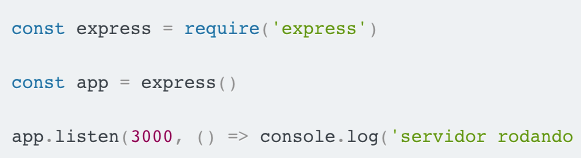
\includegraphics[width=65mm]{resources/aula2_1.png}\\
            \tiny{\textbf{Fonte:} O autor}

      \end{columns}
    \end{frame}
    %----------------------------------------------------------------
     \begin{frame}[label=lists]{Execute seu projeto}
    Para executarmos esse servidor, no console escreveremos o comando \alert{node index.js}. \\
    Veremos a mensagem 'servidor rodando na porta 3000', como esperávamos.
    \vspace{0.5cm}

	Se acessarmos no navegador o caminho \alert{localhost:3000} teremos algo em execução, mas não encontramos nenhum get, afinal não criamos nenhuma rota ainda.
    \end{frame}
%------------------------------------------------------------------------
% \subsection{Referências}
%    \begin{frame}{Referências}%[allowframebreaks]
%\frametitle{Referências}
%\small
%\begin{center}
%\tiny
%\bibliographystyle{apalike}
%\bibliography{./ref_aula}
%\end{center}
%\end{frame}
  
\end{document}
